%----------------------------------------------------------------------------------------
%	SECTION 1.1
%----------------------------------------------------------------------------------------

\section{Convexity and Contracibilty}

\begin{definition}
    We call a subset $X$ of $\R^n$  \textbf{convex} if for every $x,y \in X$,
    the line segment joining  $x$ to  $y$ is convex. That is the line
    $tx+(1-t)y \in X$ for all $t \in [0,1]$.
\end{definition}

\begin{example}\label{2.4}
    The sets $\R^n$, $I^n$,  $B^n$ and  $\Delta(\R^n)$ are all convex. The
    sphere $S^{n-1}$ is not convex.
\end{example}

\begin{definition}
    We call a topological space $X$  \textbf{contracible} if $1_X$ is
    nullhomotopic.
\end{definition}

\begin{example}\label{2.5}
    \begin{enumerate}
        \item[(1)] Let $X=\{x,y\}$ together with the topolgoy $\Tc=\{\emptyset, \{x\}, X\}$.
            Then $X$ is contractible under the topology $\Tc$. We call  $X$
            together with  $\Tc$ the \textbf{Sierpinski space}.

        \item[(2)] The space $\R^n$ is contractible, but the sphere  $S^{n-1}$
            is not contractible.

        \item[(3)] Continuous images of contractible spaces need not be
            contractible.
    \end{enumerate}
\end{example}

\begin{theorem}\label{2.3.1}
    Every convex set is contractible.
\end{theorem}
\begin{proof}
    Choose $x_0 \in X$ and consider the constant map $c:X \xrightarrow{} X$ by
    $x \xrightarrow{} x_0$ for all $x \in X$. Define  $F:X \times I
    \xrightarrow{} X$ by $F(x,t)=tx_0+(1-t)x$. This map is continuous, with
    $F(x,0)=x=1_X(x)$ and $F(x,1)=x_0=c(x)$. Therefore $1_X \simeq c$.
\end{proof}

\begin{lemma}\label{2.3.2}
    If $X$ is a contractible space, and homeomorphic to a space  $Y$, then  $Y$
    is also contractible.
\end{lemma}

\begin{example}\label{3.6}
    If $X$ and  $Y$ are subspaces of  $\R^n$, with $X$ homeomorphic to $Y$, and
     $X$ convex, then  $Y$ is contractible by lemma \ref{2.3.2}, however, $Y$
     may not be convex. This shows that not all contractible spaces are convex
     spaces.
\end{example}

\begin{lemma}\label{2.3.3}
    Contractible spaces are connected.
\end{lemma}
\begin{corollary}
    Convex sets are connected.
\end{corollary}
\begin{proof}
    This follows from theorem \ref{2.3.1}.
\end{proof}

\begin{definition}
    If $X$ is a topological space, define the equivalence relation  $\sim$ on
    $X \times I$ by  $(x,t) \sim (x',t')$ if, and only if $t=t'=1$. Denote the
    equivalence classes of  $(x,t)$ as $[x,t]$. We call the quotient space
    $\faktor{X \times I}{\sim}$ the \textbf{cone} over $X$, and denote it  $CX$.
    We call the equivalence class  $[x,1]$ the \textbf{vertex} of $CX$.
\end{definition}

\begin{figure}[h]
    \centering
    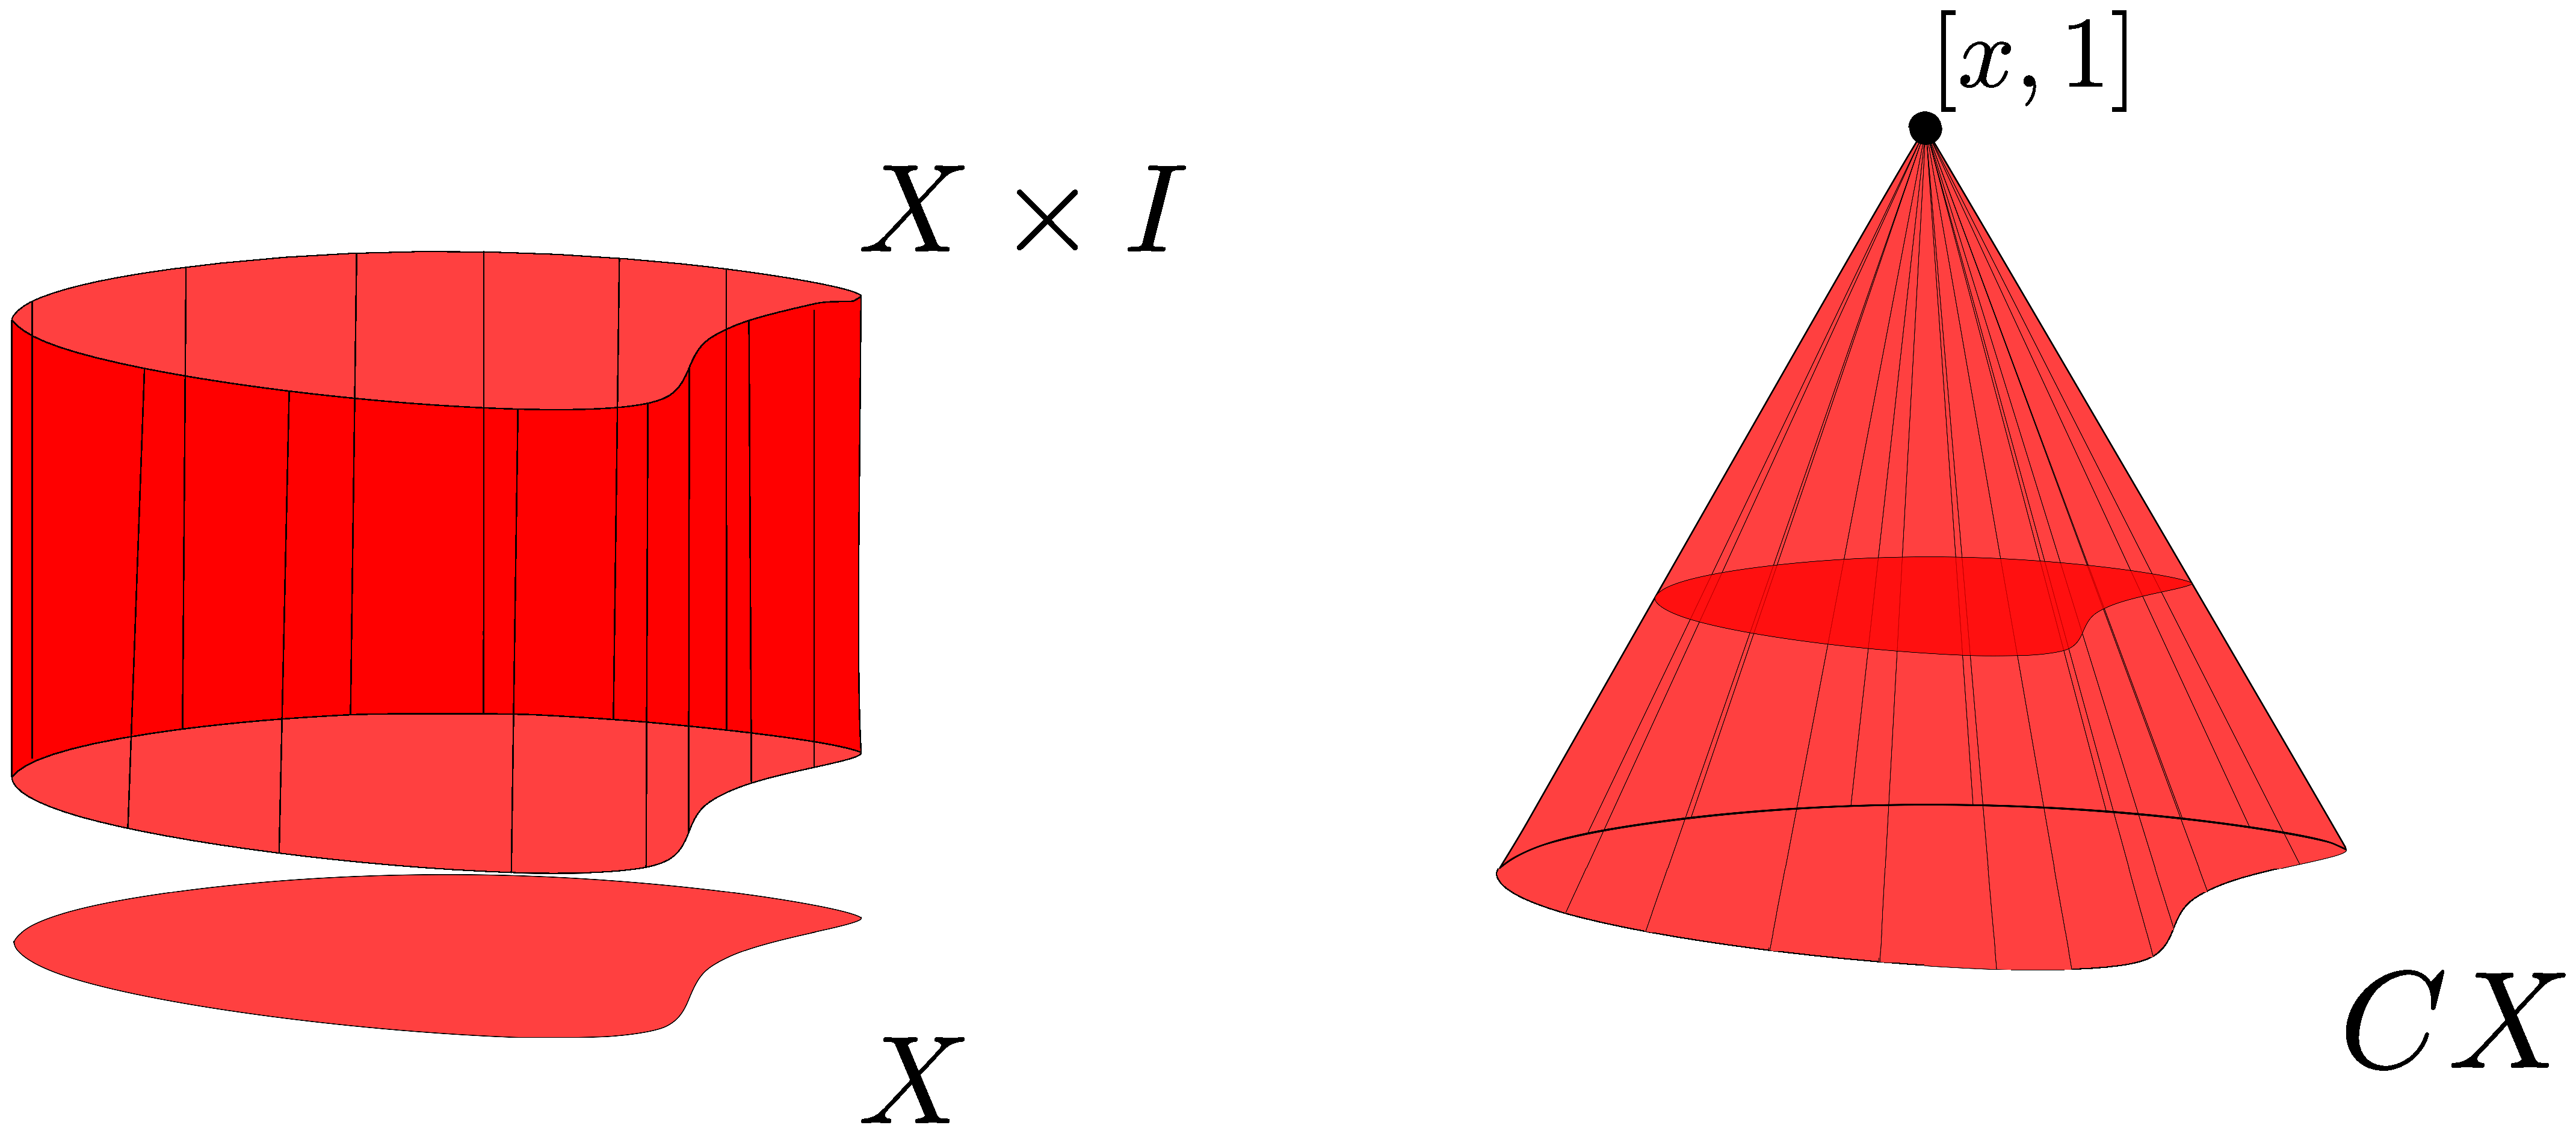
\includegraphics[scale=0.2]{Figures/Chapter3/cone.eps}
    \caption{The space $X$ and the cone $CX$ formed by identifying all $t=1$ of
    $X \times I$ to a point.}
    \label{fig_3.1}
\end{figure}

\begin{example}\label{2.7}
    \begin{enumerate}
        \item[(1)] For topological spaces $X$ and  $Y$, every continuous map  $f:X \times I
            \xrightarrow{} Y$ with $f(x,1)=y_0$ for some $y_0 \in Y$ induces a
            continuous map $Cf:CX \xrightarrow{} Y$ by taking $[x,t] \xrightarrow{}
            f(x,t)$.

        \item[(2)] The cone over $S^{n-1}$ is $CS^{n-1}=D^n$ and has the vertex
            $0$.
    \end{enumerate}
\end{example}

\begin{theorem}\label{2.3.4}
    For any topological space $X$, the cone over  $X$ is contractible.
\end{theorem}
\begin{proof}
    Define the map $F:CX \times I \xrightarrow{} CX$ by taking $([x,t],s)
    \xrightarrow{} [x,(1-s)t+s]$. This map is continuous by composition,
    moreover $F([x,t],0)=[x,t]$ and $F([x,t],1)=[x,1]$ which makes $1_{CX}
    \simeq c$ where $c:CX \xrightarrow{} CX$ is the constant map taking $[x,t]
    \xrightarrow{} [x,1]$ for all $x \in X$.
\end{proof}

\begin{theorem}\label{2.3.5}
    A topological space has the same homotopy type as a point if, and only if
    $X$ is contractible.
\end{theorem}
\begin{proof}
    Let $\{a\}$ be a point space, and suppose that $X \simeq \{a\}$ have the
    same homotopy type. Then there are maps $f:X \xrightarrow{} \{a\}$ and
    $g:\{a\} \xrightarrow{} X$ with $a \xrightarrow{g} x_0$ such that  $g \circ
    f \simeq 1_X$ and  $f \circ g \simeq 1_{\{a\}}$. Notice that $g \circ
    f(x)=g(a)=x_0$, for all $x \in X$, so  $g \circ f$ is constant. This makes
    $1_X$  (and $1_Y$) nullhomotopic. Therefore $X$ is contractible.

    On the otherhand, supposing that  $X$ is contractible, let  $1_X \simeq c$
    where  $c:X \xrightarrow{} X$ is the constant map defined by $x
    \xrightarrow{} x_0$ for all $x \in X$. Define the maps  $f:X \xrightarrow{}
    \{x_0\}$ and  $g:\{x_0\} \xrightarrow{} X$ by $x \xrightarrow{f} x_0$ and
    $x_0 \xrightarrow{g} x_0$. Observe that $g \circ f=1_X$, and that $f
    \circ g \simeq 1_{\{x_0\}}$ Therefore $X$ is of the same homotopy type as
    $\{x_0\}$.
\end{proof}
\begin{remark}
    This theorem shows that the simplest objects in $\hTop$ are the contractible
    spaces.
\end{remark}

\begin{theorem}\label{2.3.6}
    If $Y$ is a contractible space, then any two maps  $X \xrightarrow{} Y$ are
    homotopic.
\end{theorem}
\begin{proof}
    Suppose that $1_Y \simeq c$ where  $c:Y \xrightarrow{} Y$ takes $y
    \xrightarrow{} y_0$ for all $y \in Y$. Defie $g:X \xrightarrow{} Y$ by
    taking $x \xrightarrow{} y_0$ for all $x \in X$. If  $f:X \xrightarrow{} Y$
    is any continuous map, then $f \simeq g$. Consider the diagram
    \[\begin{tikzcd}
        X && Y && Y
        \arrow[from=1-1, to=1-3]
        \arrow["k", curve={height=-6pt}, from=1-3, to=1-5]
        \arrow["{1_Y}"', curve={height=6pt}, from=1-3, to=1-5]
    \end{tikzcd}\]
    Since $1_Y \simeq k$, we get that  $f=1_Y \circ f \simeq k \circ f=g$.
\end{proof}
\begin{corollary}
    Any two maps $X \xrightarrow{} Y$ are nullhomotopic.
\end{corollary}
